\documentclass[11pt, a4paper]{article}
\usepackage{graphicx} % Required for inserting images
\usepackage{caption} % for captions
\usepackage{bbm} % Math font; use \mathbbm{}
\usepackage[acronym]{glossaries} % for acronyms
\usepackage{physics} % Physics symbols

\usepackage{showlabels} % To show equations labels on the PDF. Comment at the end

% Defining acronyms
\newacronym{etk}{ETK}{Einstein Toolkit}

% Defining variables
\newcommand\figifcap{Initial and final conditions}
\newcommand\figrescompcap{Resolution comparison}

\title{Numerical Relativity Homework 2}
\author{Federico Leto di Priolo}
\date{June 2024}

\begin{document}

\maketitle

\section{Sod Shock Tube Problem}

The Sod shock tube problem consists of a one-dimensional Riemann
problem with initial discontinuities in density and pressure. The time
evolution of the system can be computed by solving the Euler equations.
Since the solution to this problem can be computed exactly, it is useful
for testing the accuracy of numerical codes. In this exercise, we solve
the Sod problem with the \acrfull{etk} using different resolutions and
compare the results with the exact solution.

The solution to the problem is described by three characteristics, each
related to the propagation speed of the fluid in different
regions. These can be associated with either a rarefaction wave, a shock
wave, or a contact discontinuity. Specifically, the pressure and the
velocity of the fluid develop a rarefaction wave and a shock wave, while
the density also develops a contact discontinuity. The exact solution
along with the initial conditions is shown in Figure
\ref{fig:all_exact_if}.

For the numerical solutions, the HLLE Riemann solver has been used, along
with the Minmod slope limiter. The domain extends in the range
\([-0.5, 0.5]\), and the evolution proceeds up to time \(t = 0.4\).
The grid spacings used are \(\{0.005, 0.0025, 0.00125, 0.000625\}\),
corresponding respectively to \(\{200, 400, 800, 1600\}\) grid points.

\subsection{Highest Resolution: 1600 points}

We will use the results obtained with the highest resolution to showcase
how the numerical solutions look. Figure
\ref{fig:all_1600_snapshots} shows some snapshots of the profiles of
density, pressure, and velocity of the fluid, including the initial and
the final ones. As can be seen, S and CD waves travel in opposite
directions with respect to the R waves. We point out that the fact that
the initial profile in Figure \ref{fig:all_1600_snapshots} doesn't
perfectly resemble a step (as it should) is due to the way the
numerical results are interpolated on the chosen uniform grid
\([-0.45, 0.45]\). Interpolation effects are also present in the final
profile, though they are less evident. Figure
\ref{fig:all_1600_initial_compare} compares the interpolated initial
data with the raw initial data actually used by the \acrshort{etk}.

The numerical solution manages to correctly capture the discontinuities
in the observed physical variables for the Sod problem. The accuracy
depends on the number of grid points, but the slight smoothing
of the discontinuities seems to be a characteristic feature of the
HLLE Riemann solver. This doesn't seem to be related to the
interpolation of the data on the plot's grid, as shown in the next
section (Section \ref{sec:rescomp}).

\subsection{Resolutions Comparison} \label{sec:rescomp}

Now we look at the results obtained with different resolutions and
compare them to the exact solution. In order to avoid visualization
artifacts, we will use the raw data from the \acrshort{etk} and not the
interpolated ones. Figures \ref{fig:rho_final_rescompare},
\ref{fig:press_final_rescompare}, and \ref{fig:vel_final_rescompare}
show the final iteration of the evolution of, respectively, density,
pressure, and velocity.
As mentioned in the previous section, the smoothing of the
discontinuities appears to be a feature of the Riemann solver rather
than of the chosen resolution. At the same time, as expected, it is
indeed true that a finer spacing of the numerical grid reduces the
observed smoothing.

\newpage

\begin{center}
    \centering
    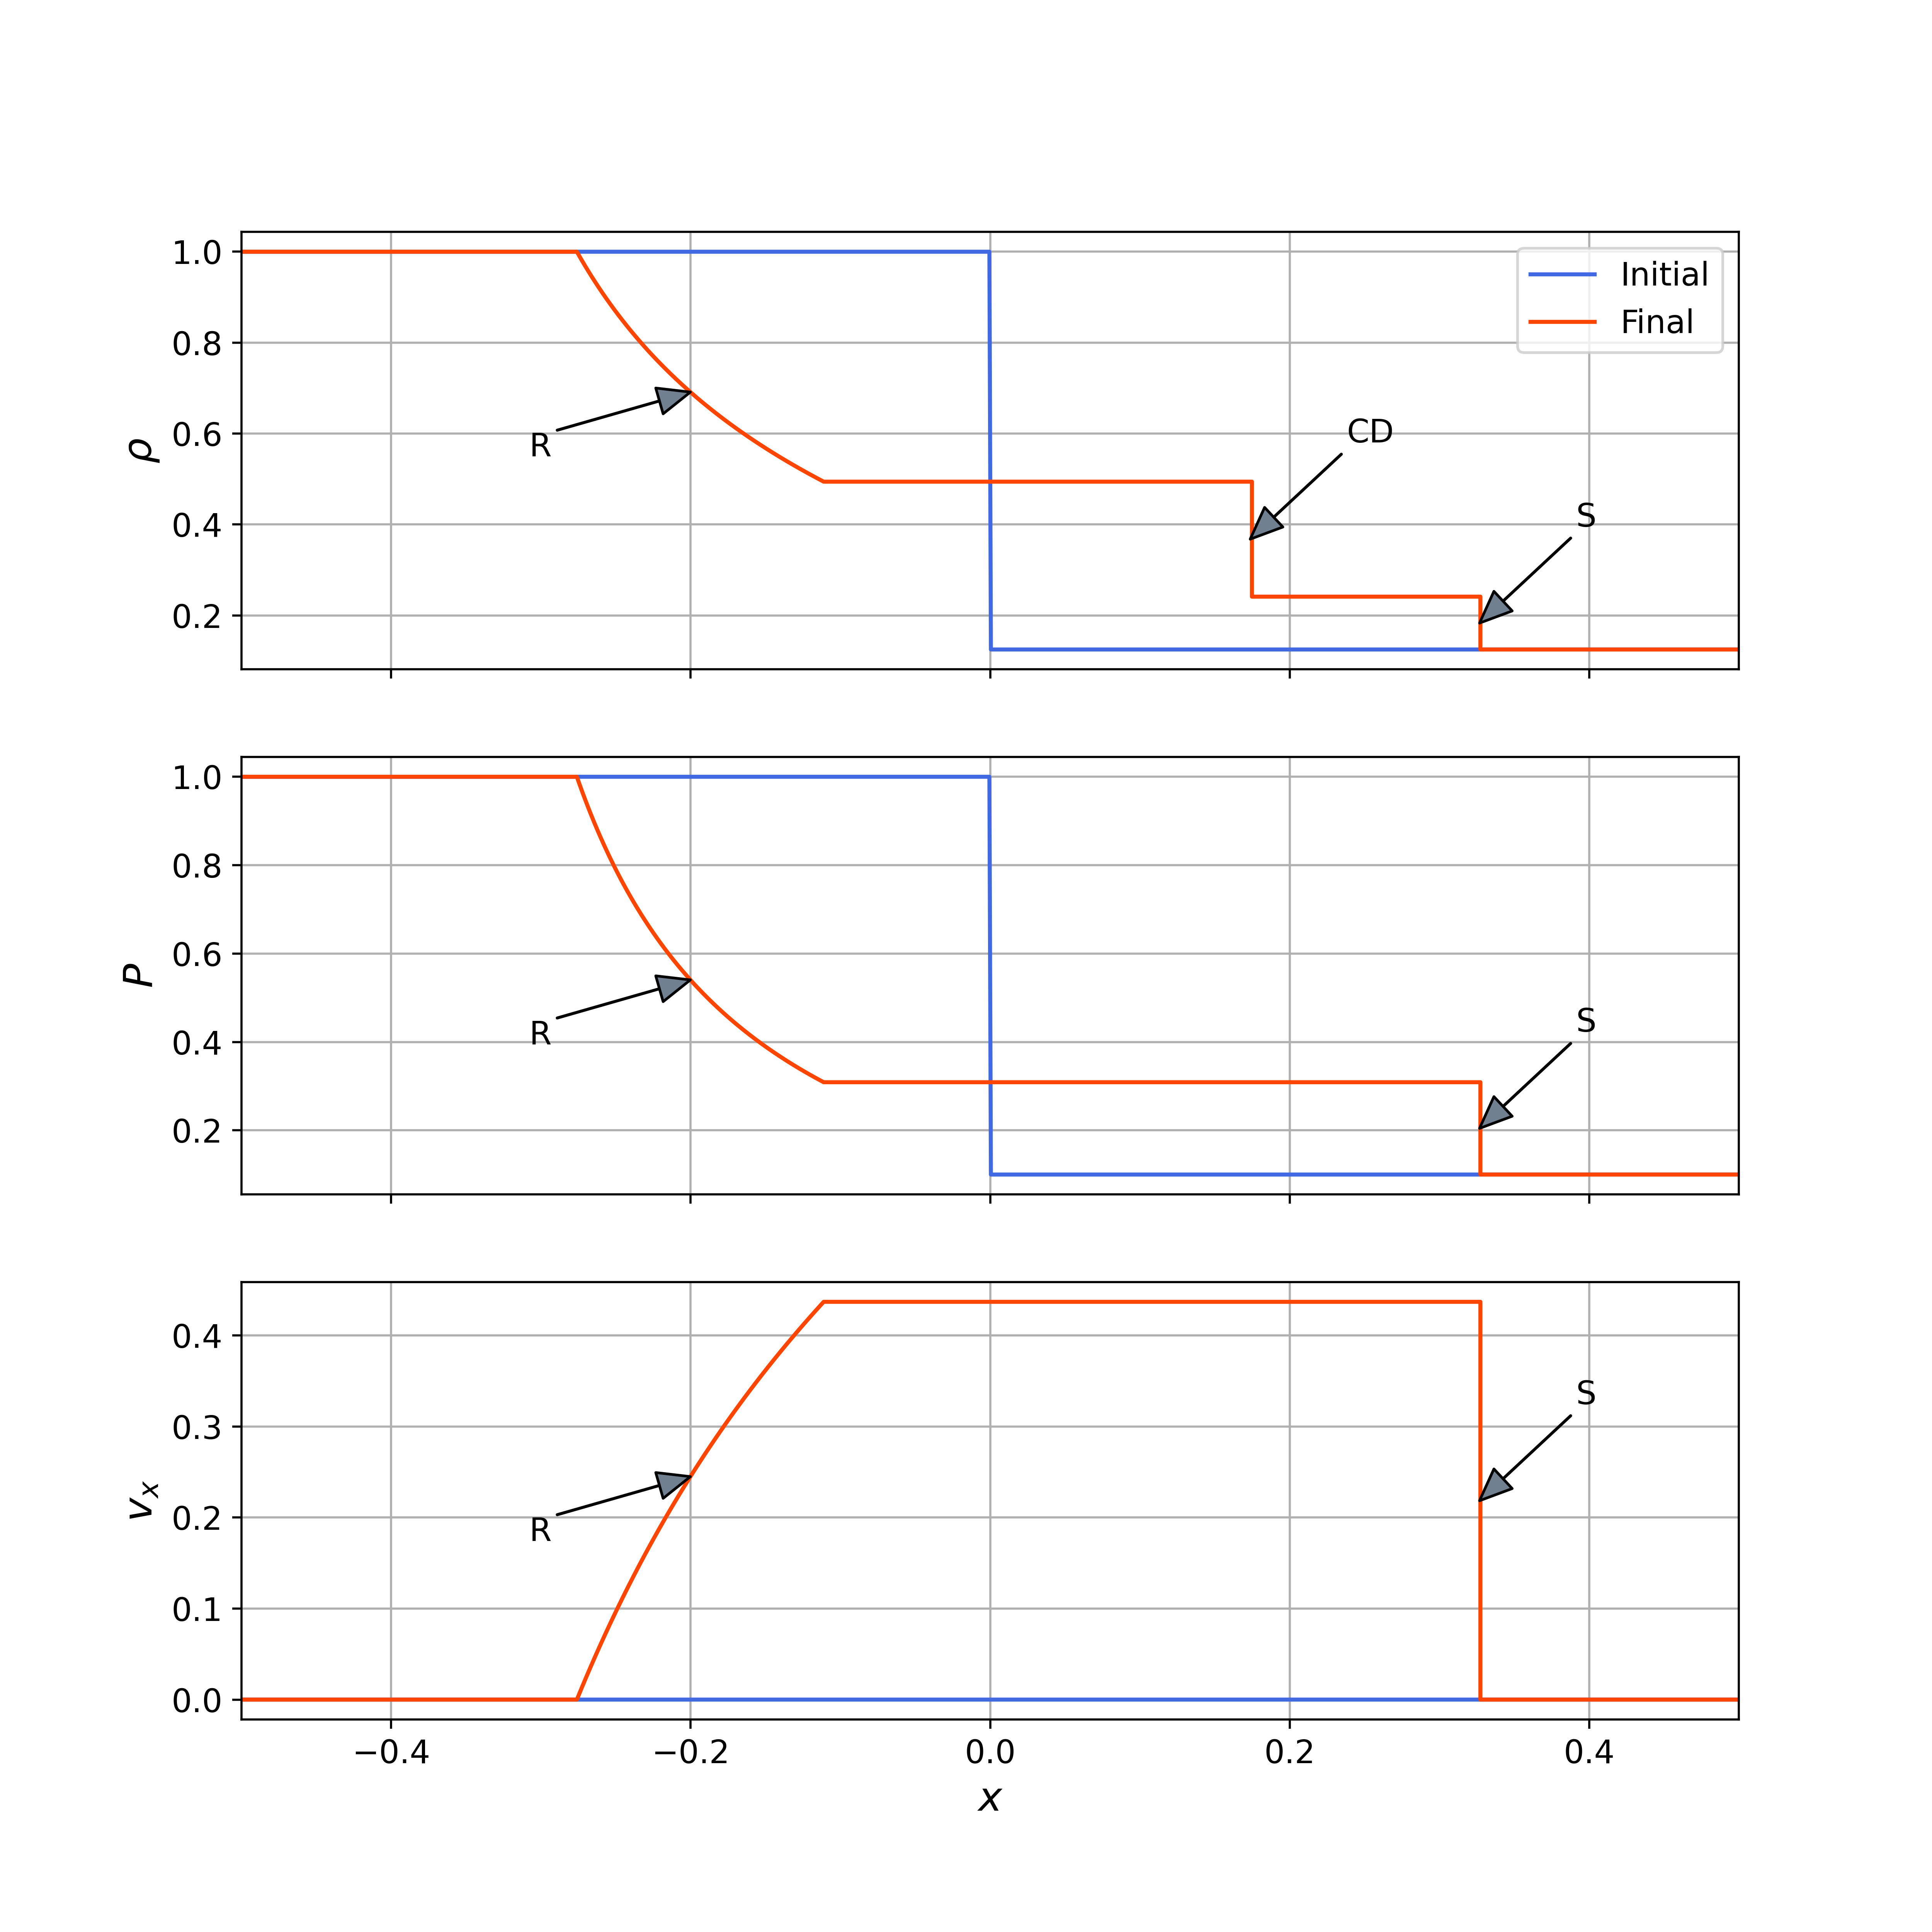
\includegraphics[width=1\linewidth]{images/all_exact_if.png}
    \captionof{figure}{Exact Solution; \figifcap; The arrows points at the different types of waves: R (Rarefaction), S (Shock) and CD (Contact Discontinuity).}
    \label{fig:all_exact_if}
\end{center}

\begin{center}
    \centering
    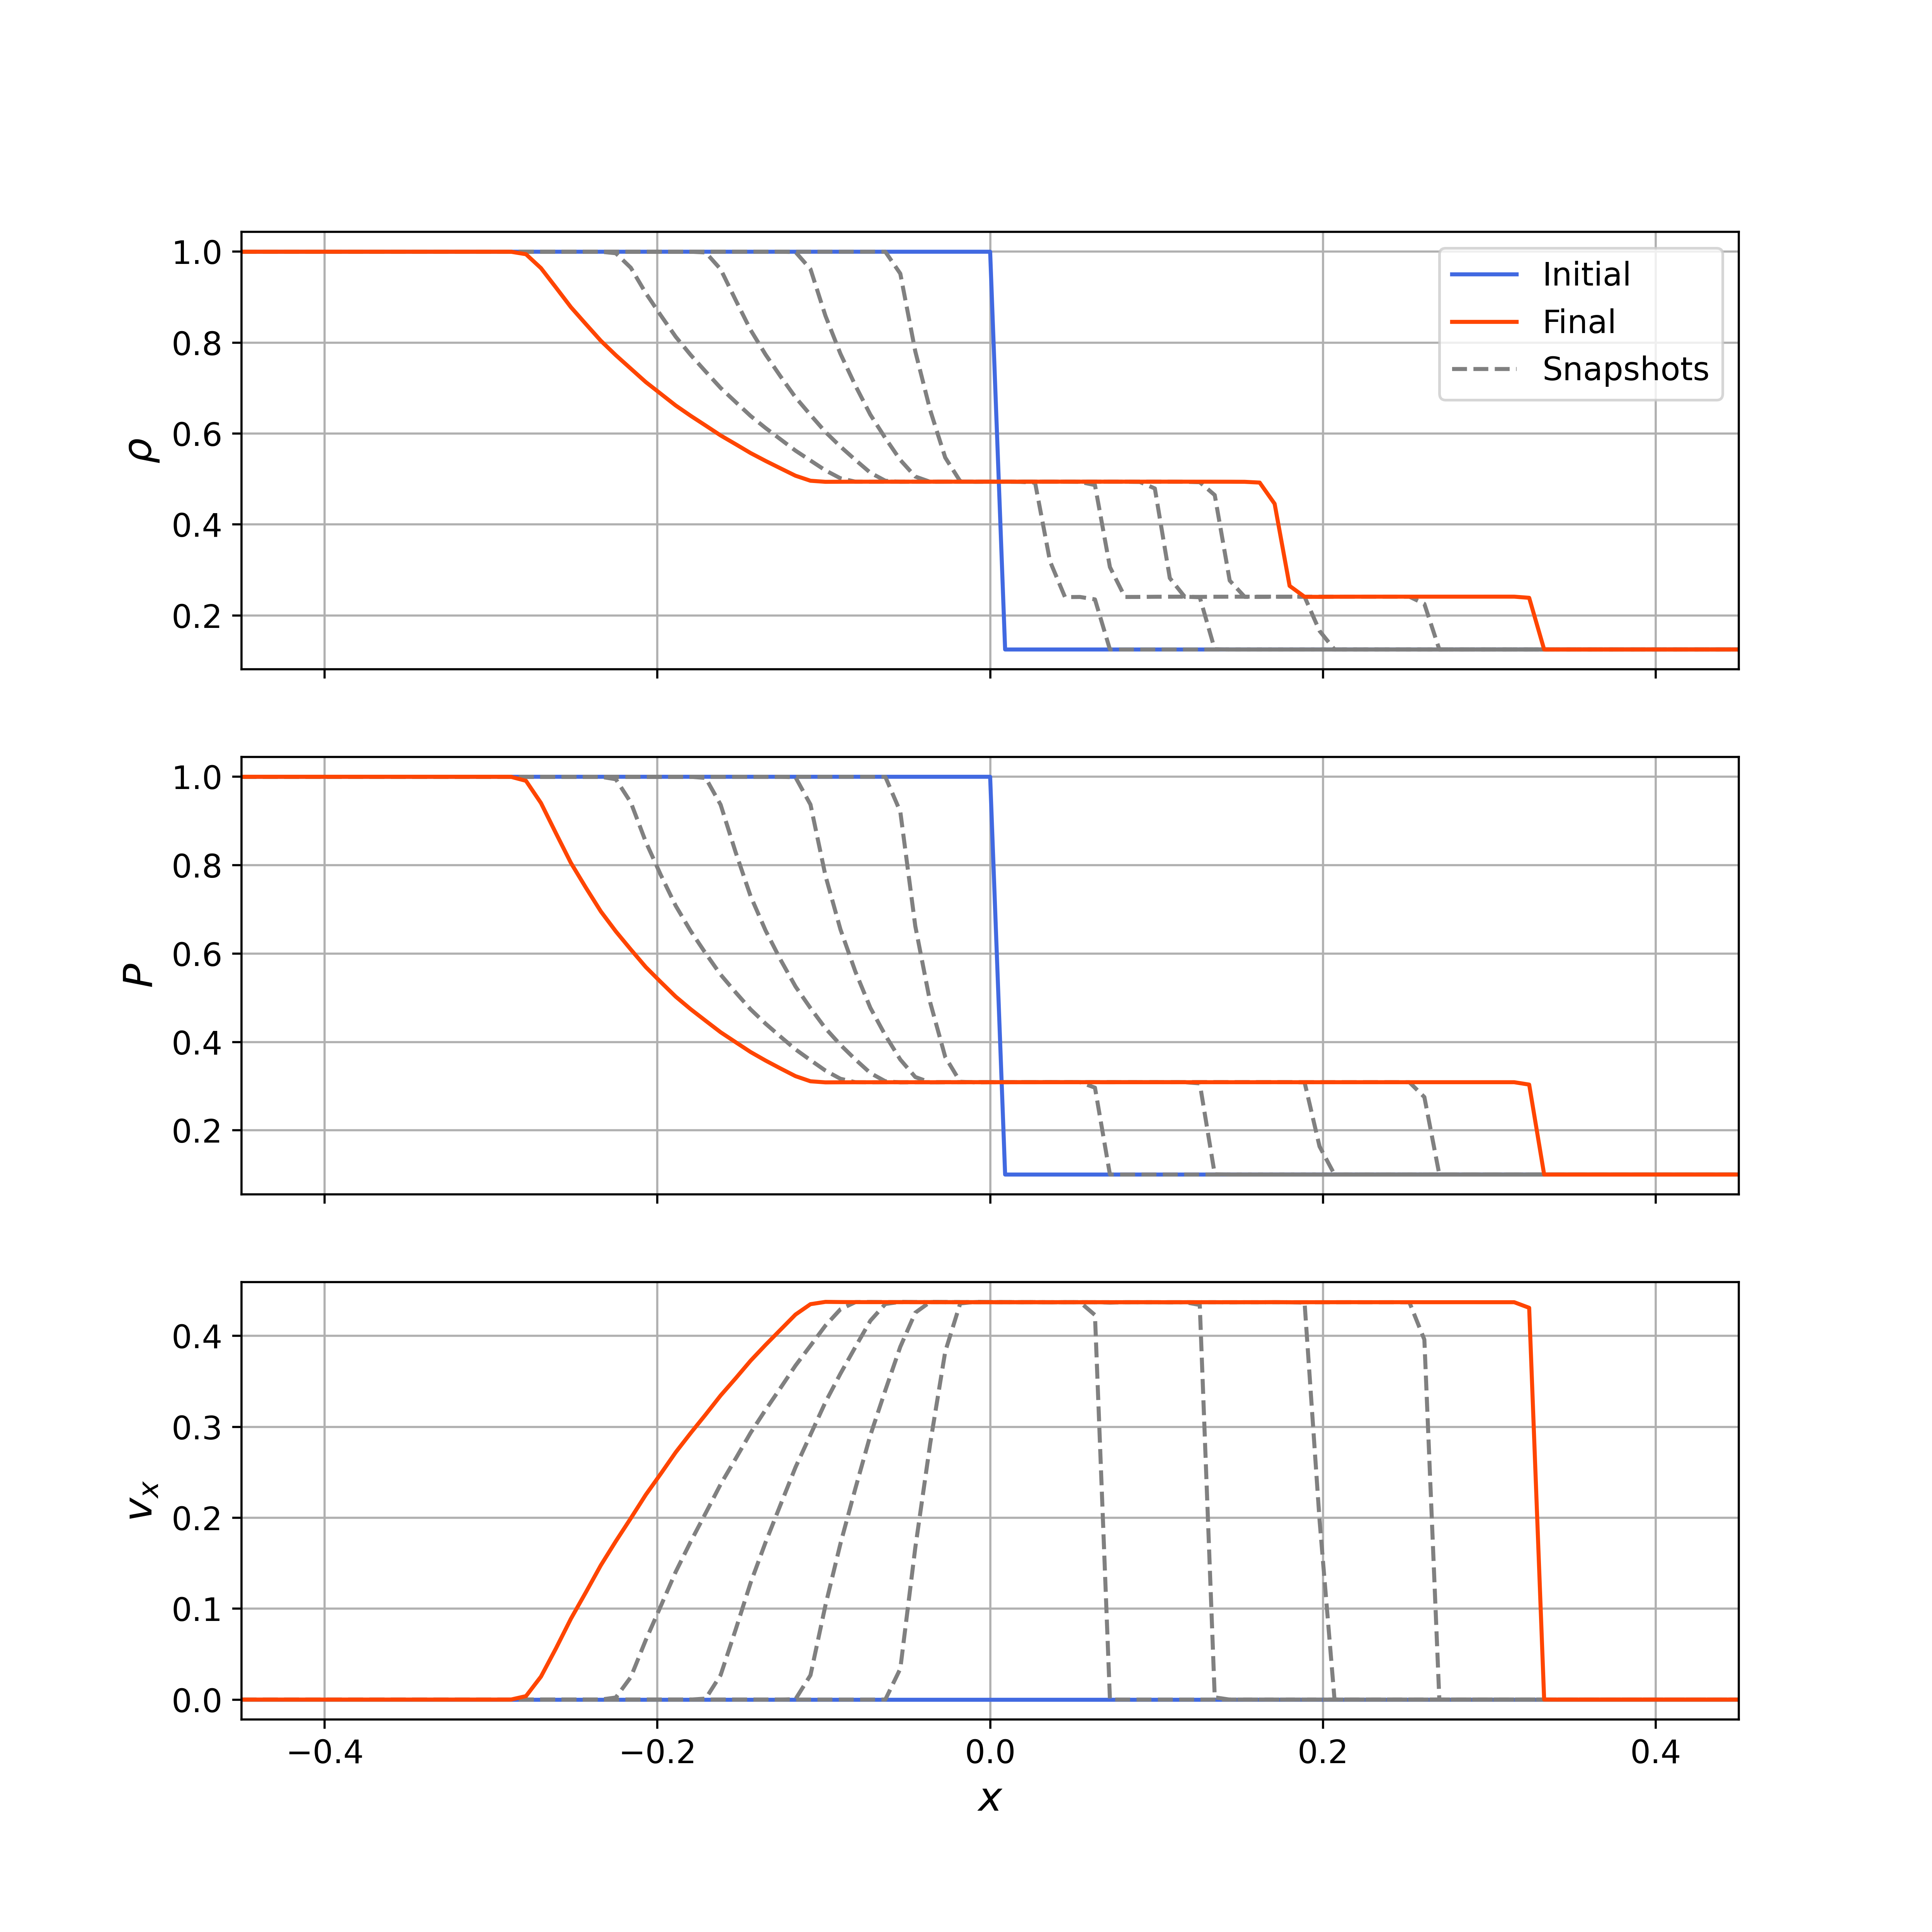
\includegraphics[width=1\linewidth]{images/all_1600_snapshots.png}
    \captionof{figure}{Numerical Solution; 1600 points; Snapshots.}
    \label{fig:all_1600_snapshots}
\end{center}

\begin{center}
    \centering
    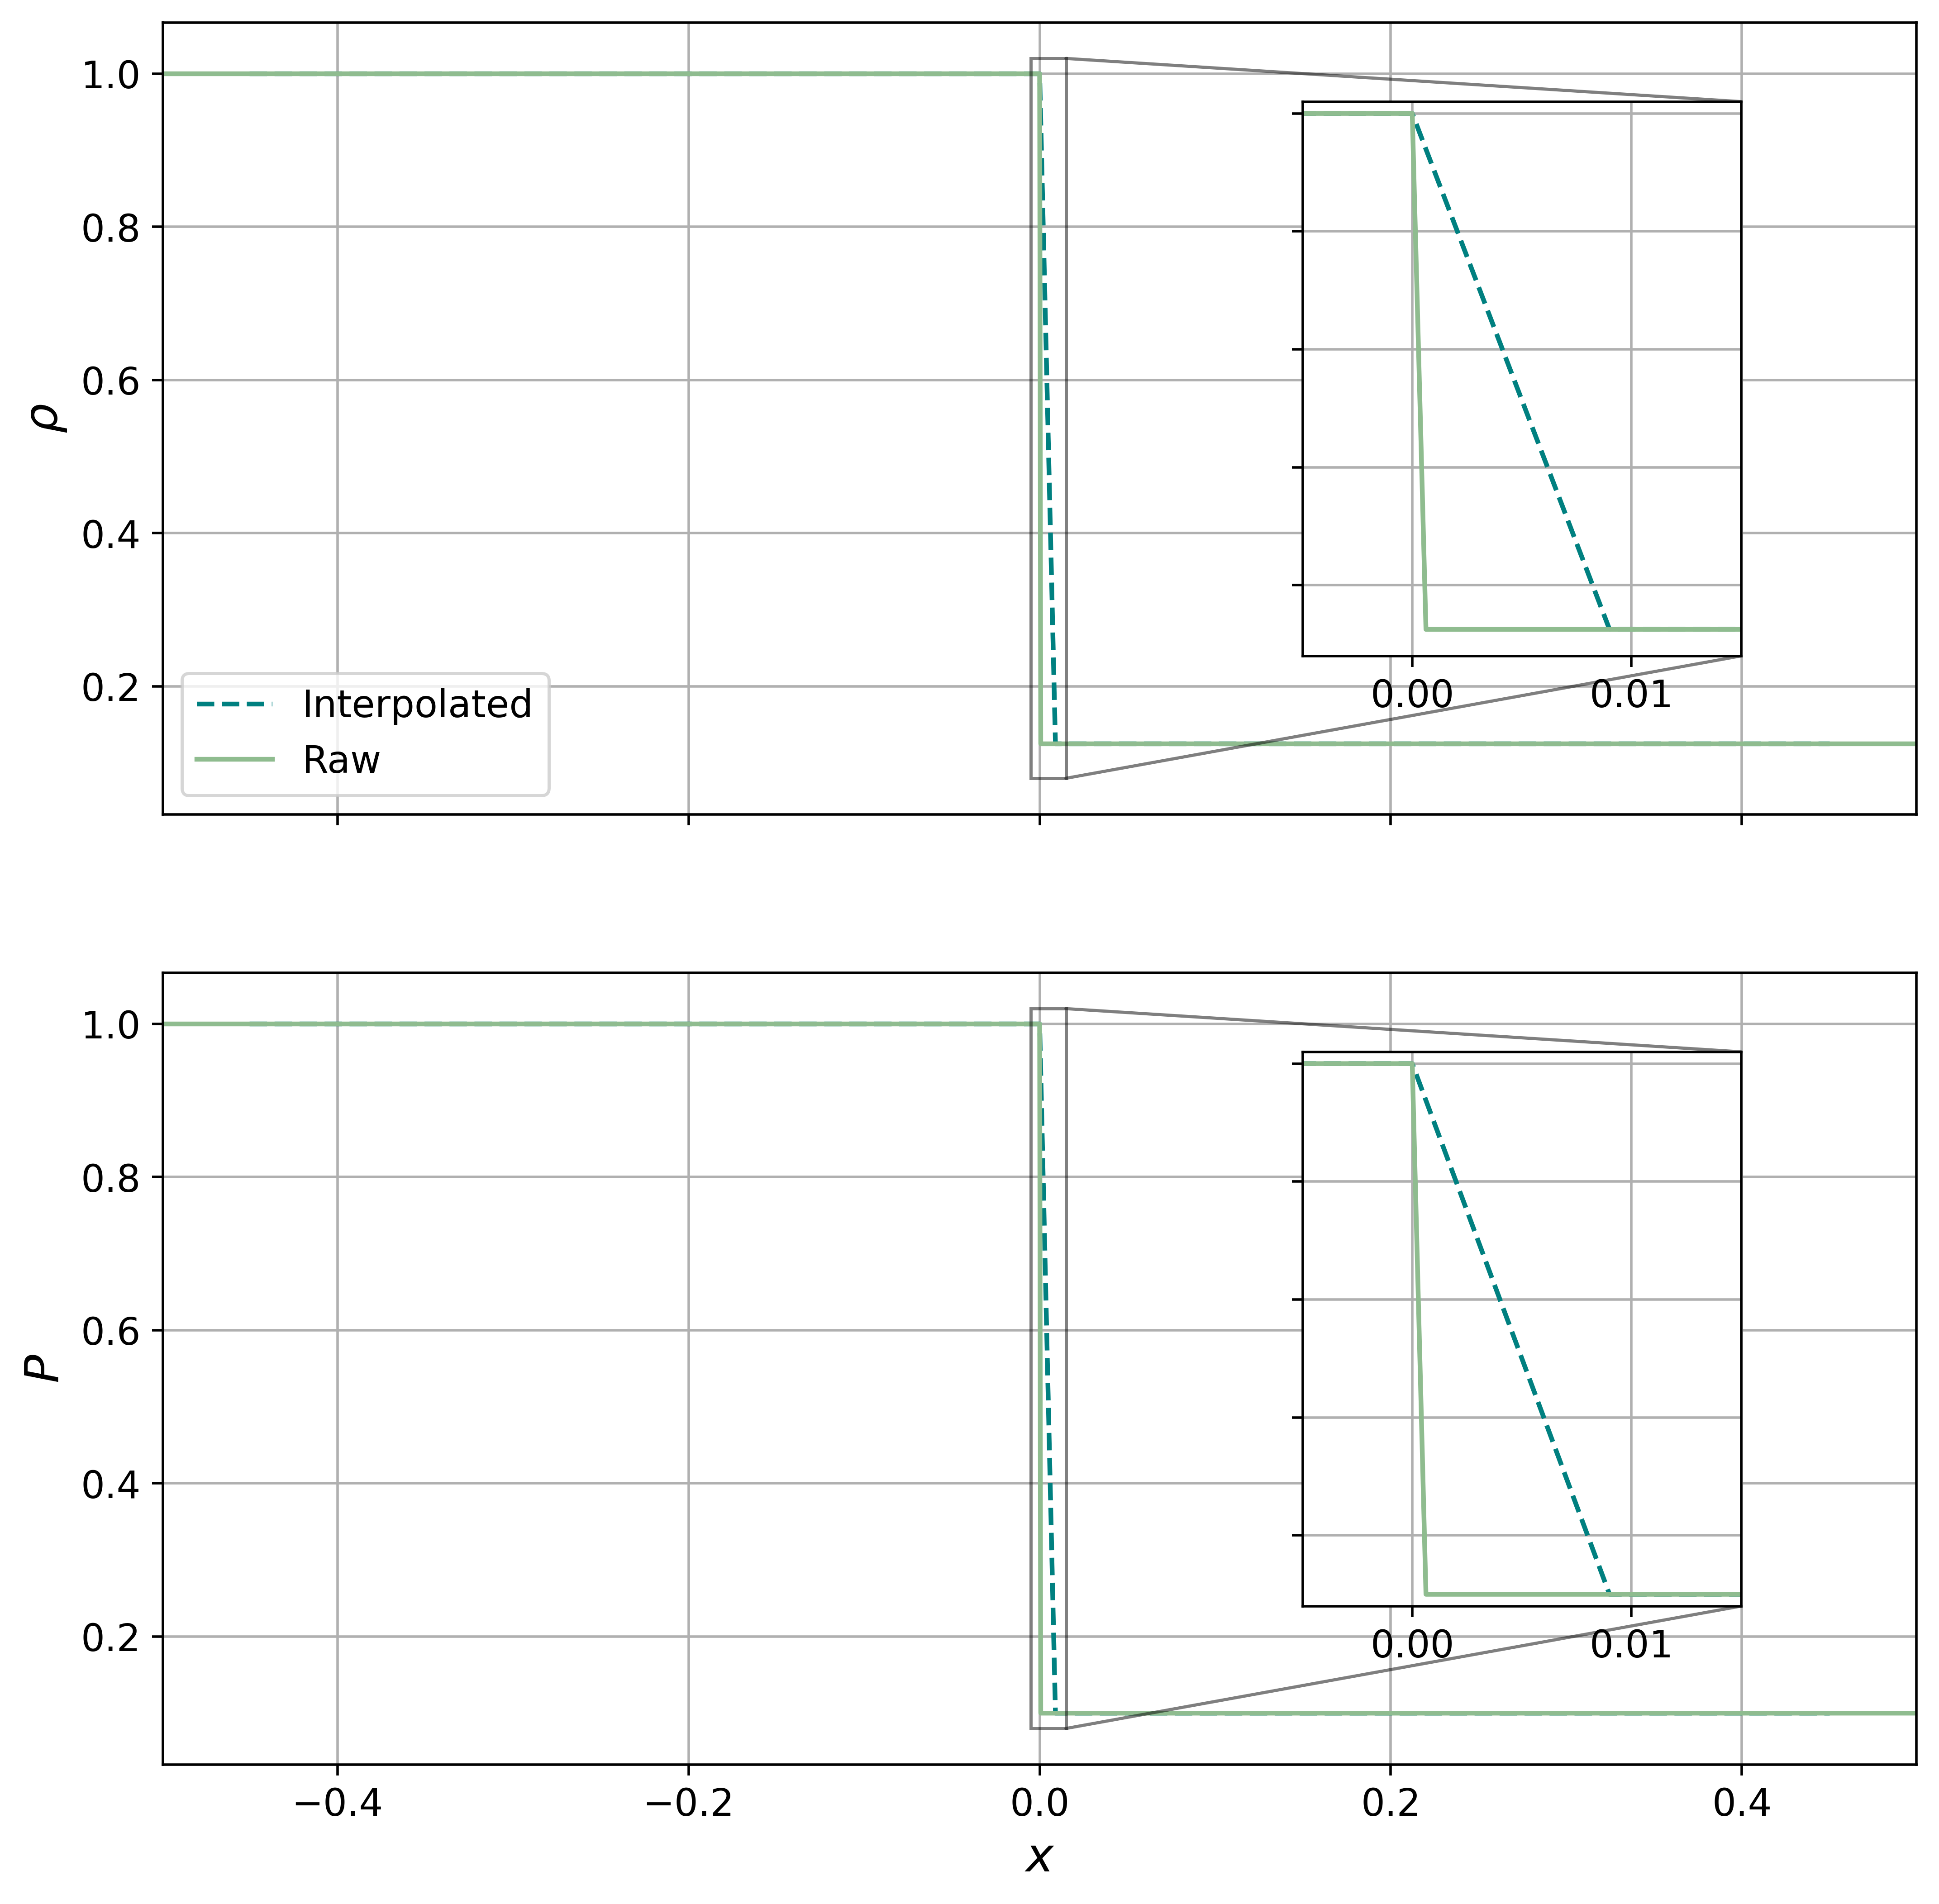
\includegraphics[width=1\linewidth]{images/all_1600_initial_compare.png}
    \captionof{figure}{Initial data; 1600 points; Raw and interpolated.}
    \label{fig:all_1600_initial_compare}
\end{center}

\begin{center}
    \centering
    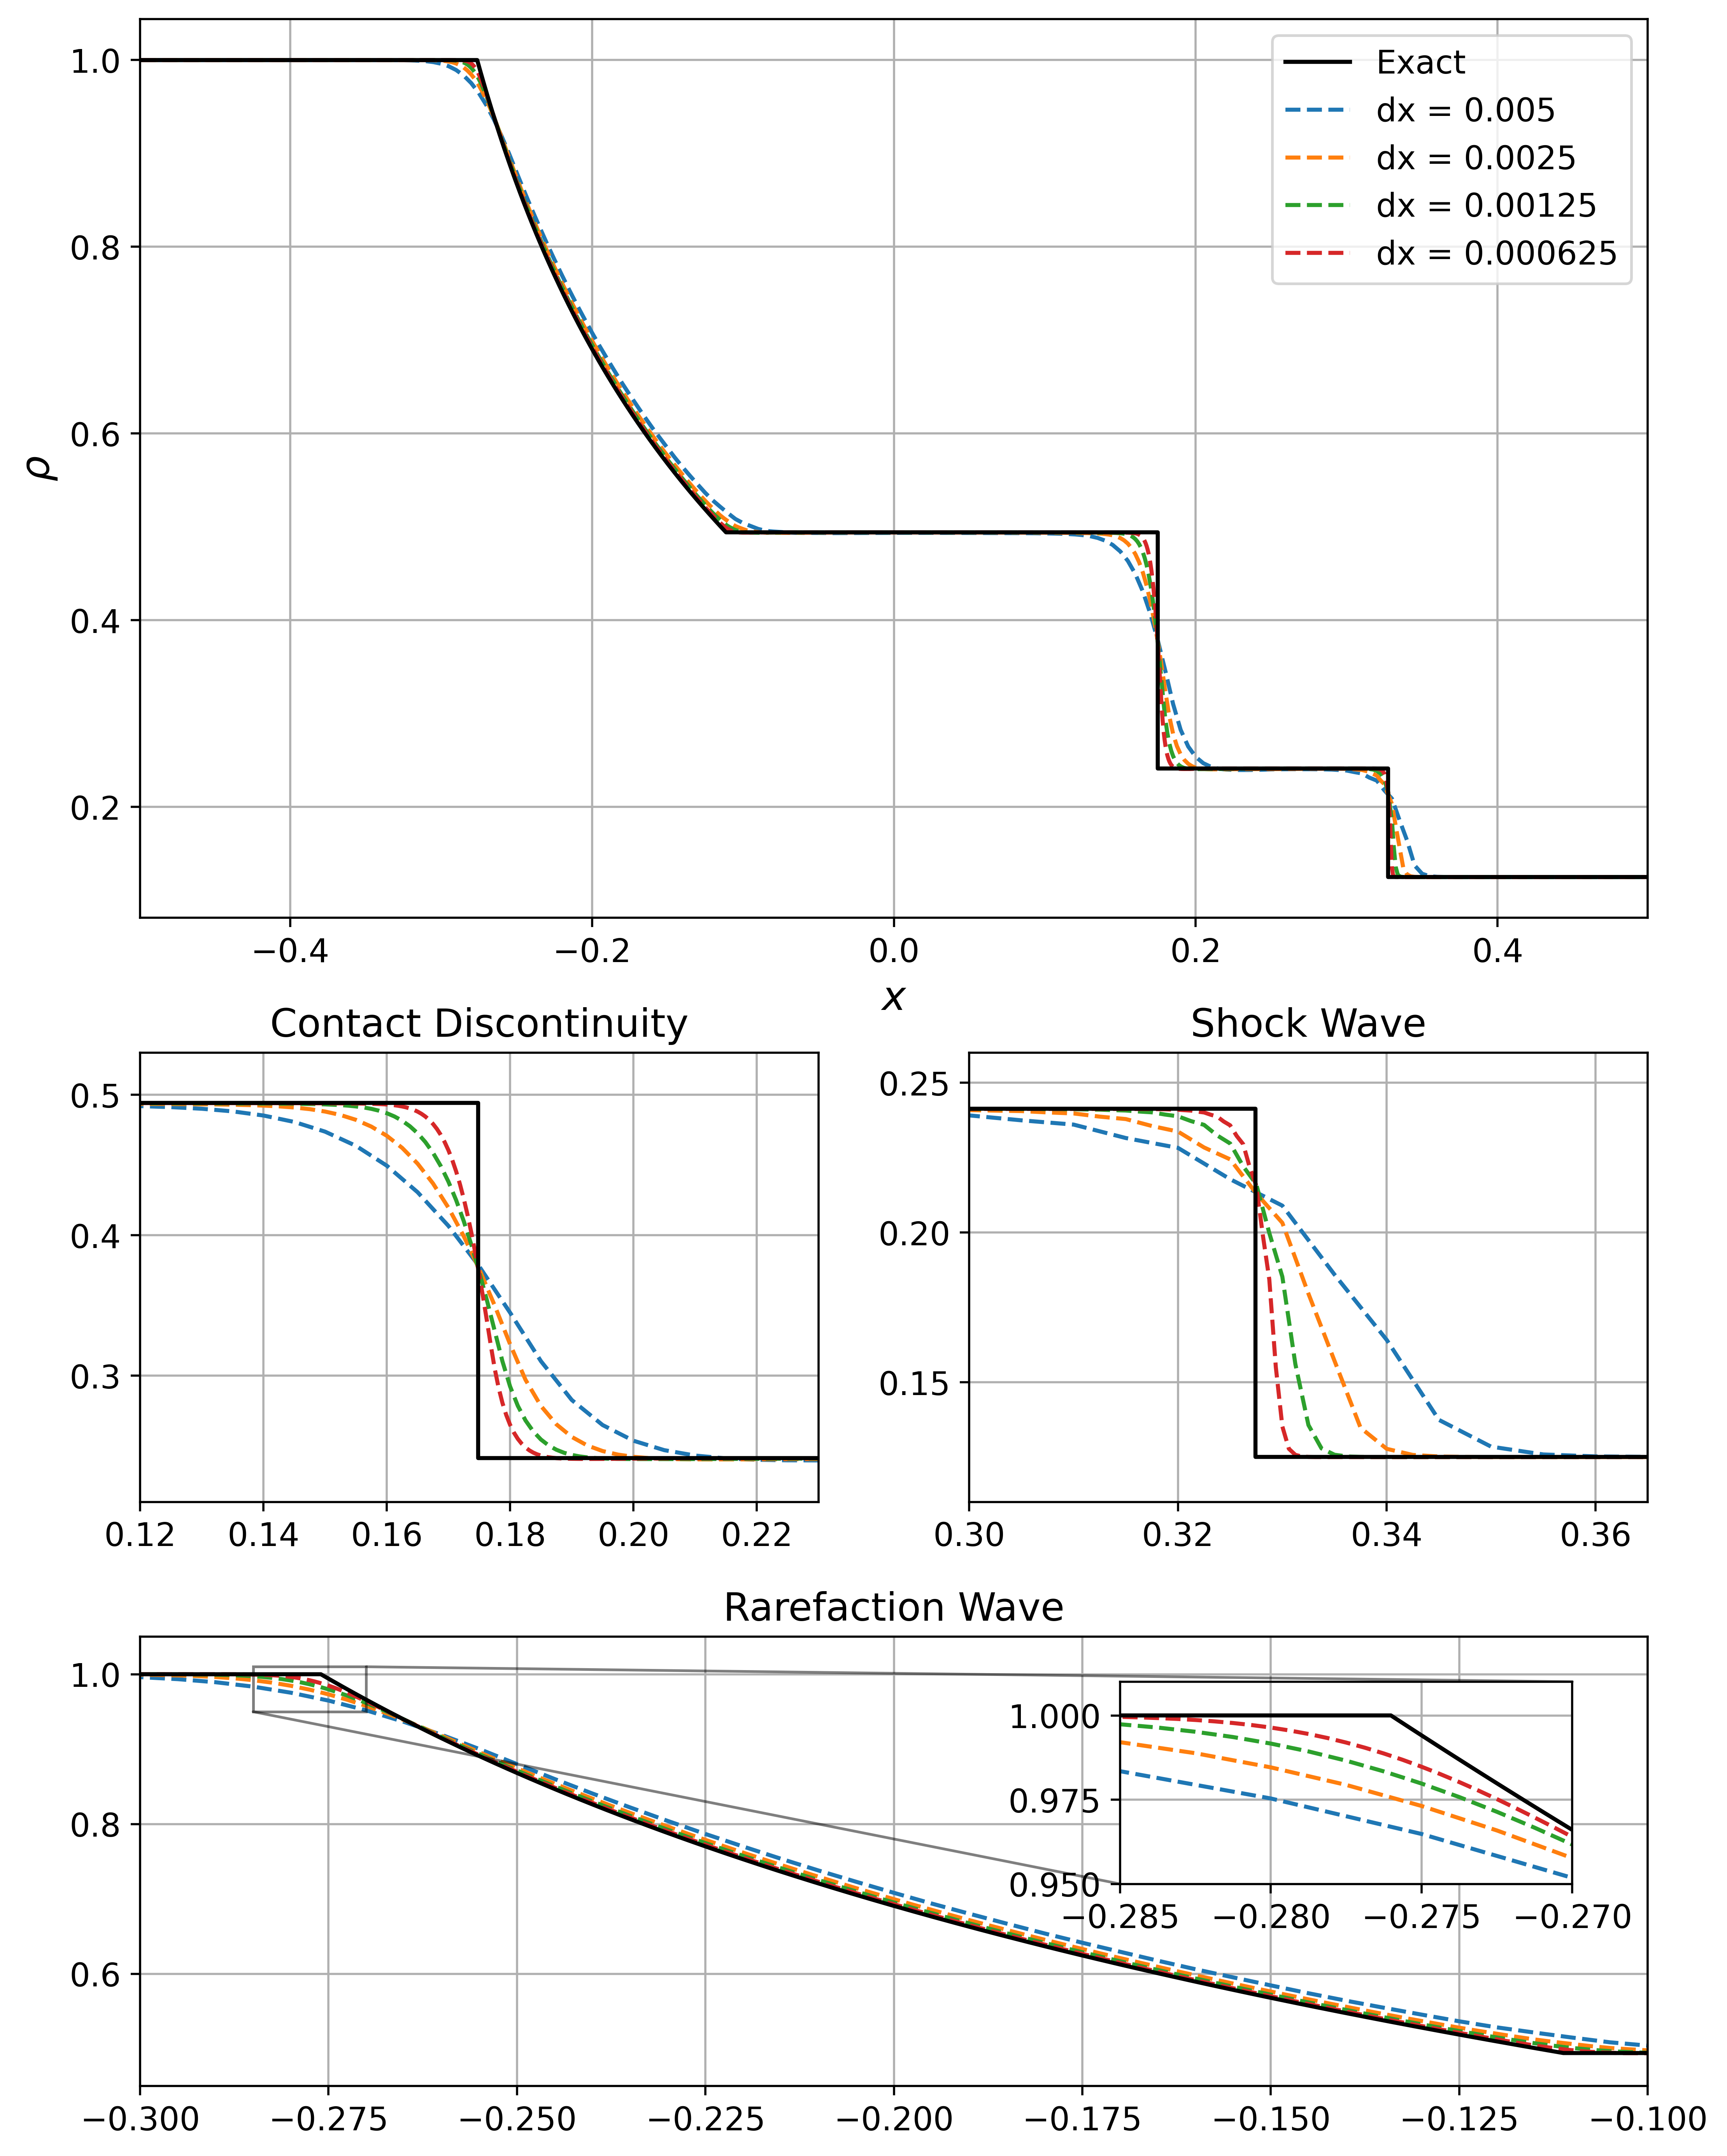
\includegraphics[width=1\linewidth]{images/rho_final_rescompare_raw.png}
    \captionof{figure}{Density; Final data; \figrescompcap.}
    \label{fig:rho_final_rescompare}
\end{center}

\begin{center}
    \centering
    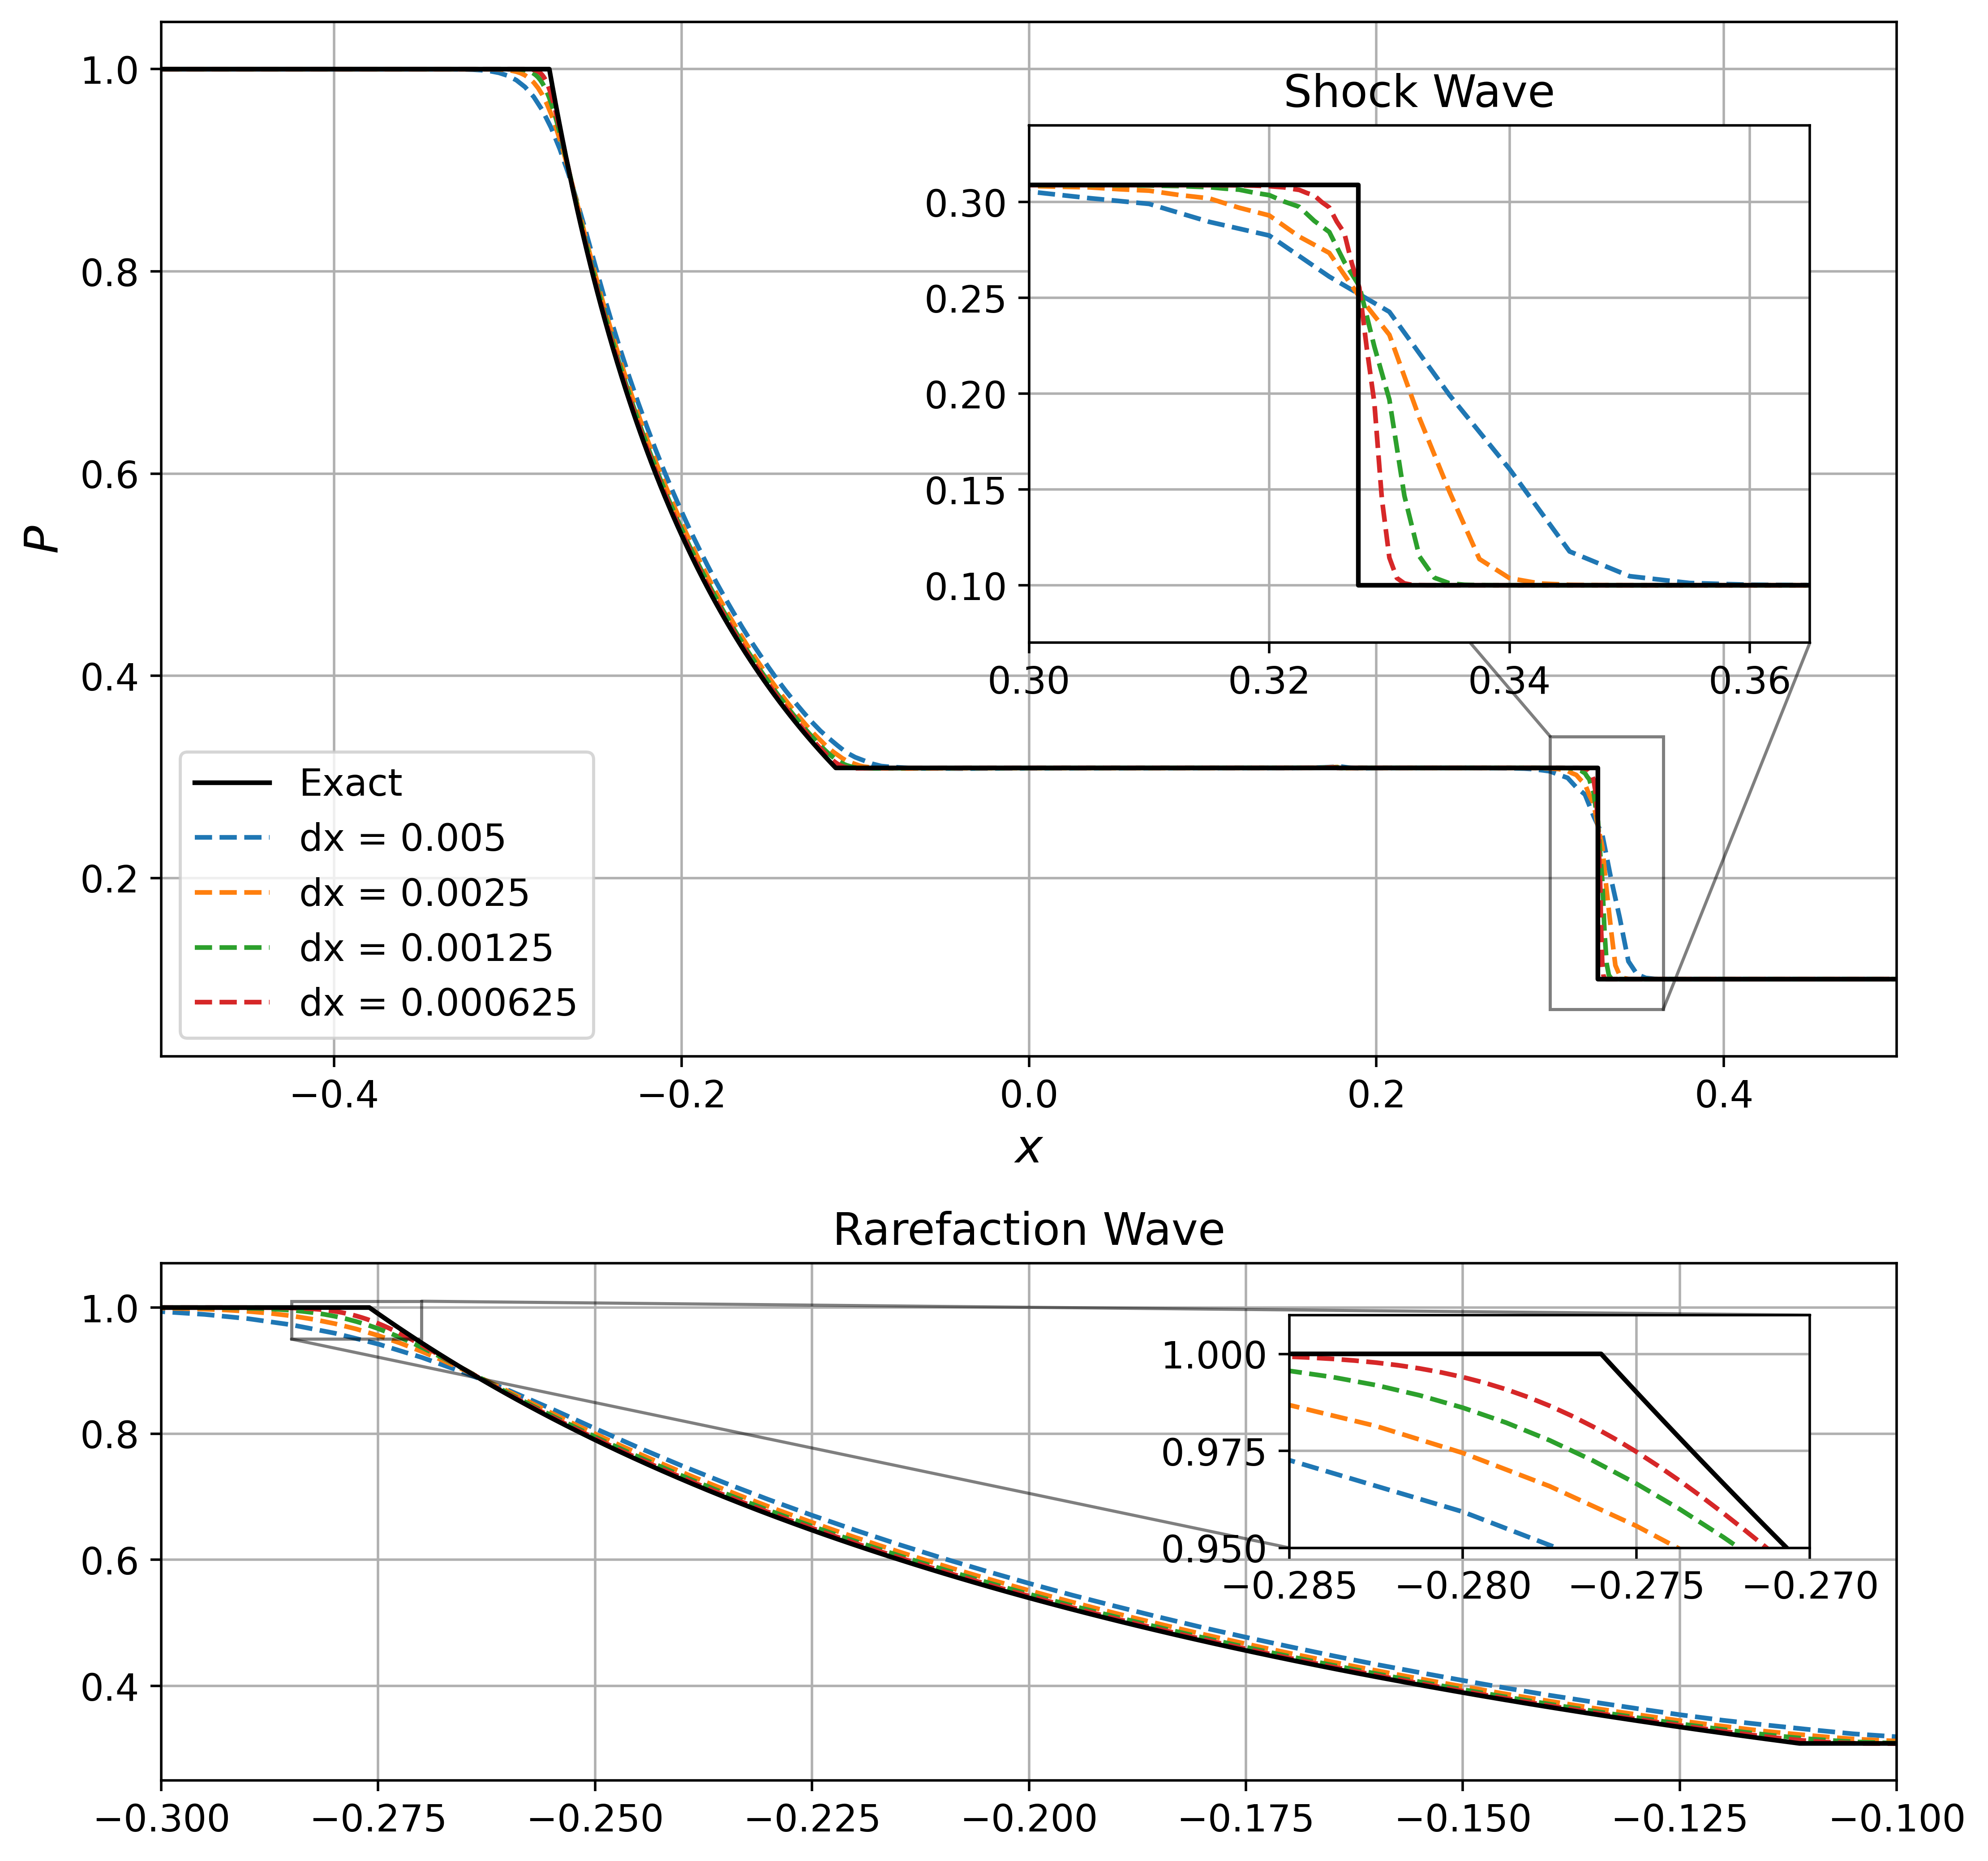
\includegraphics[width=1\linewidth]{images/press_final_rescompare_raw.png}
    \captionof{figure}{Pressure; Final data; \figrescompcap.}
    \label{fig:press_final_rescompare}
\end{center}

\begin{center}
    \centering
    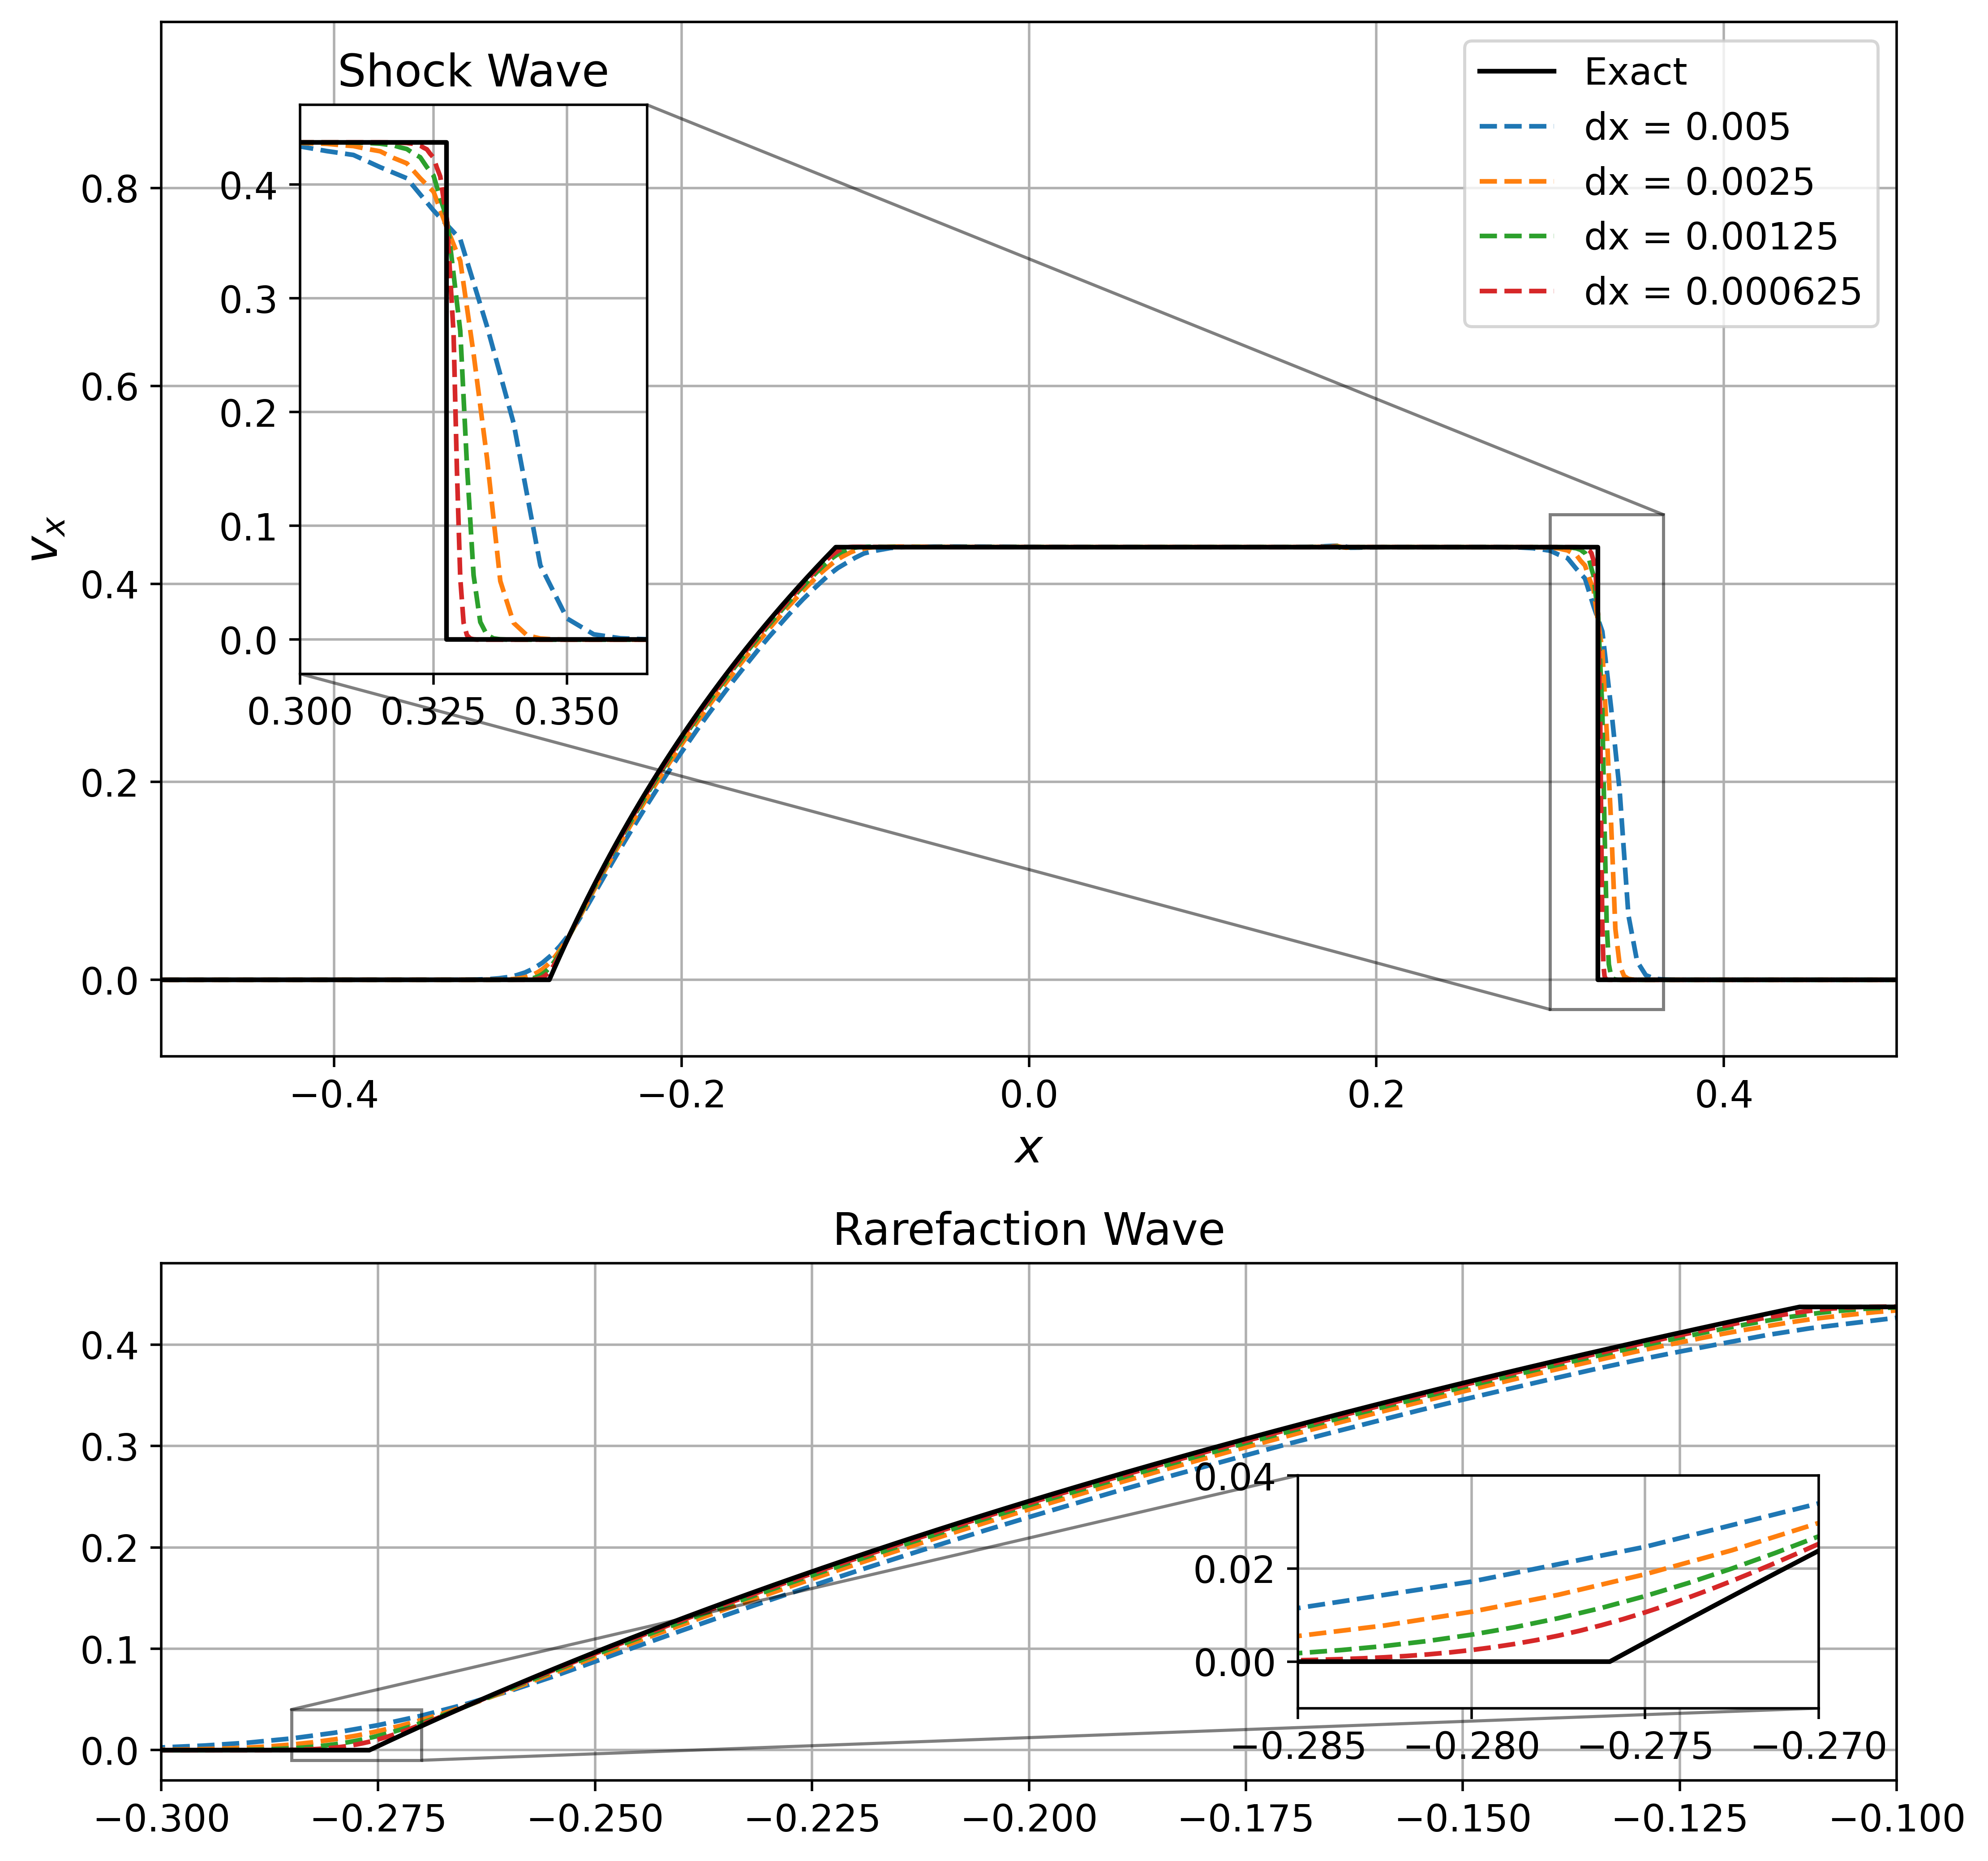
\includegraphics[width=1\linewidth]{images/vel[0]_final_rescompare_raw.png}
    \captionof{figure}{Velocity; Final data; \figrescompcap.}
    \label{fig:vel_final_rescompare}
\end{center}

\newpage

\section{TOV Evolution}

\end{document}
